\chapter{Βιβλιογραφική Επισκόπηση}
\label{chap:related_work}

Πριν την έναρξη της εκπόνησης του πρακτικού τμήματος της παρούσας διπλωματικής πραγματοποιήθηκε βιβλιογραφική επισκόπηση προκειμένου να αναζητηθούν εργασίες σχετικές με το θέμα των νευρωνικών δικτύων με κάψουλες. Στο κεφάλαιο αυτό, θα γίνει αναφορά στις σημαντικότερες από αυτές οι οποίες λήφθηκαν υπόψιν και ενέπνευσαν τις μεθόδους που θα αναλύσουμε στο επόμενο κεφάλαιο. \par

Αρχικά, θα παρουσιάσουμε τις τρεις βασικές δημοσιεύσεις των \en{Hinton G. et al.} \cite{hinton2011transforming, sabour2017dynamic, hinton2018matrix} που θεμελίωσαν τη θεωρία πίσω από τα νευρωνικά δίκτυα με κάψουλες σε ένα πλαίσιο επιβλεπομένης μάθησης. Έπειτα, θα αναφερθούμε στις ποικίλες παραλλαγές αυτών, όπως προκύπτουν από την τροποποίηση της αρχιτεκτονικής ή του αλγορίθμου δρομολόγησης. Στη συνέχεια, θα γίνει λόγος για τα νευρωνικά δίκτυα με κάψουλες σε περιβάλλον μη\textendash επιβλεπομένης μάθησης. Τέλος, θα αναλυθούν συνοπτικά εργασίες οι οποίες δεν εντάσσονται άμεσα στις ανωτέρω κατηγορίες αλλά βοηθούν είτε άμεσα είτε έμμεσα στην αποτελεσματική επίλυση του γενικότερου προβλήματος της γενίκευσης σε νέες οπτικές γωνίες.\par

Συγκεντρωτικά, μέσα από την παρακάτω βιβλιογραφική μελέτη αντλούμε τα εξής χρήσιμα συμπεράσματα:
\begin{itemize}
    \item Οι βασικές υλοποιήσεις των \en{Hinton G. et al.} εμφανίζουν ορισμένες ιδιότητες (π.χ. ευρωστία σε μετασχηματισμούς περιστροφής και σε επικαλυπτόμενα αντικείμενα) οι οποίες και ταυτοποιούν την αρχιτεκτονική των νευρωνικών δικτύων με κάψουλες. Συνεπώς, κάθε νέα αρχιτεκτονική που ισχυρίζεται ότι αποτελείται από κάψουλες οφείλει να υποβάλλεται σε δοκιμές που αποδεικνύουν την παρουσία των χαρακτηριστικών ιδιοτήτων (σύνολα δεδομένων \en{affNIST} και \en{MultiMNIST}).
    \item Πολλές από τις υλοποιήσεις των νευρωνικών δικτύων με κάψουλες (συμπεριλαμβανομένων των \cite{hinton2011transforming, sabour2017dynamic, hinton2018matrix}) βασίζονται στις υποθέσεις που παρουσιάστηκαν στην ενότητα \ref{sec:core_assumptions}. Παρόλα αυτά, στη βιβλιογραφία δεν εντοπίστηκαν εκτενή πειράματα που ελέγχουν την εγκυρότητα των υποθέσεων.
    \item Αρκετές υλοποιήσεις επιδιώκουν να βελτιώσουν τον αλγόριθμο δρομολόγησης με συμφωνία με σκοπό να είναι ταχύτερος ή να οδηγεί σε καλύτερα πειραματικά αποτελέσματα. Αρκετές από αυτές τις προτάσεις δε διενεργούν εκτενή πειράματα ώστε να πιστοποιηθεί ότι η νέα, προτεινόμενη αρχιτεκτονική σέβεται τις θεμελιακές αρχές των νευρωνικών δικτύων με κάψουλες.
    \item Η εν λόγω τεχνολογία δεν κλιμακώνει εύκολα λόγο μεγάλου υπολογιστικού κόστους. Κατά συνέπεια, οι εφαρμογές της περιορίζονται σε απλά σύνολα δεδομένων.
\end{itemize}

\section{Θεμελίωση Θεωρίας Νευρωνικών Δικτύων με Κάψουλες}

Όπως έχουμε αναφέρει, η ιδέα των νευρωνικών δικτύων με κάψουλες δεν είναι καινούρια αφού παρουσιάστηκε για πρώτη φορά από τους \en{Hinton G. et al.} το 2011. Παρόλα αυτά, σχετικά πρόσφατα, μετά από διαδοχικές δημοσιεύσεις, ωρίμασε και πέτυχε αξιοσημείωτα αποτελέσματα σε σύνολα δεδομένων όπως το \en{MultiMNIST}\cite{sabour2017dynamic}. Στην ενότητα αυτή θα κάνουμε λόγο για τα πρώτα τρία βασικά έργα πάνω στην εν λόγω αρχιτεκτονική τεχνητών νευρωνικών δικτύων. Πιο αναλυτικά, θα ξεκινήσουμε από τη δημοσίευση στην οποία πρωτοπαρουσιάστικε η ιδέα και θα καταλήξουμε στην πιο σύνθετη έκδοση των νευρωνικών δικτύων με κάψουλες για επιβλεπόμενη μάθηση που με τις επιδόσεις της στο σύνολο δεδομένων \en{smallNORB}\cite{lecun2004learning} κέντρισε το ενδιαφέρον των ερευνητών. 

\subsubsection{\en{Transforming Autoencoders}}

Στο έργο των \en{Hinton G. et al.}\footnote{Σε ελεύθερη μετάφραση: \textquote{Αυτο\textendash κωδικοποιητές Μετασχηματισμού}.} \cite{hinton2011transforming} παρουσιάζεται για πρώτη φορά η ιδέα των νευρωνικών δικτύων με κάψουλες. Η ιδέα απορρέει από την παρατήρηση ότι οι παρούσες μέθοδοι αναγνώρισης αντικειμένων σε εικόνες είναι ανεπαρκείς (για τους λόγους που αναφέραμε στην ενότητα \ref{sec:capsule_theory}). Έτσι, προκειμένου να γίνεται αποδοτικότερη αναγνώριση αντικειμένων (σε νέες οπτικές γωνίες), προτείνεται η αρχιτεκτονική του \textquote{αυτο\textendash κωδικοποιητή μετατροπέα} (\en{transforming auto\textendash encoder}). Η αρχιτεκτονική αυτή αποτελείται από ένα επίπεδο από \textquote{κάψουλες}, όπως φαίνεται στο σχήμα \ref{fig:trans_autoencoder}\footnote{Στην πρώιμη μορφή τους, οι κάψουλες διέφεραν από τη γενική μορφή που περιγράψαμε στην προηγούμενη ενότητα.}.\par

\begin{figure}[h]
    \centering
    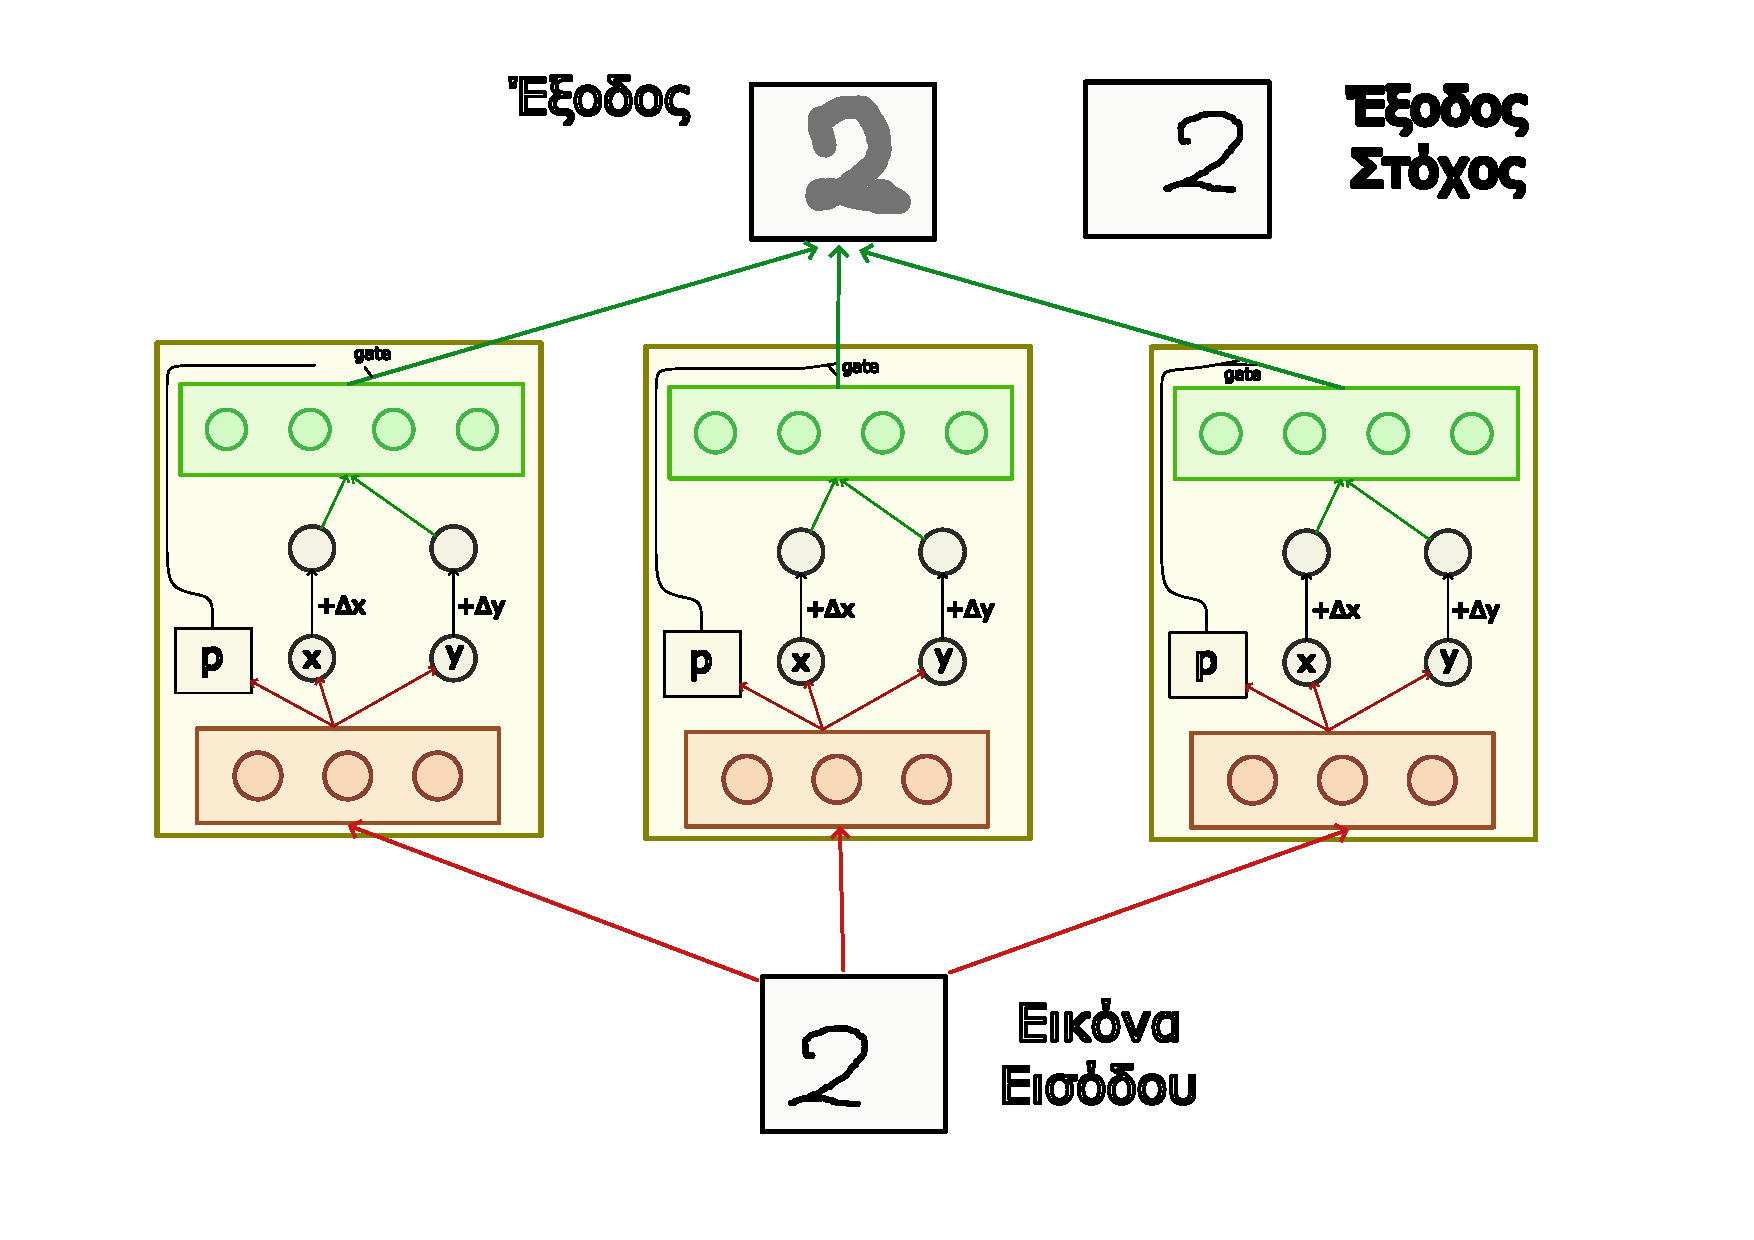
\includegraphics[width=0.8\textwidth]{images/chapter realted work/transforming_auto_gr.pdf}
    \caption{Αρχιτεκτονική αυτο\textendash κωδικοποιητών μετασχηματισμού \textit{Παράχθηκε από το \href{https://inkscape.org/}{\en{Inkscape}}}.}
    \label{fig:trans_autoencoder}
\end{figure}

Κάθε κάψουλα αποτελείται από τις \textquote{μονάδες αναγνώρισης} (\en{recognition units}) οι οποίες παράγουν τις παραμέτρους στιγμιοτύπου καθώς και μια τιμή που συμβολίζει την πιθανότητα η οντότητα που αναγνωρίζει η κάψουλα να είναι παρούσα στο οπτικό της πεδίο (στο τμήμα της εικόνας εισόδου με το οποίο συνδέονται οι μονάδες αναγνώρισής της \textemdash στην περίπτωσή μας, σε ολόκληρη την εικόνα). Οι μονάδες παραγωγής είναι υπεύθυνες και για τον μετασχηματισμό από τον χώρο εικονοστοιχείων της εικόνας εισόδου σε έναν χώρο όπου οι μετασχηματισμοί οπτικής γωνίας (μετατόπισή, περιστροφή κ.α.) είναι γραμμικοί. Στη συνέχεια, κάθε κάψουλα τροφοδοτείται με τους καθολικούς (\en{global}) μετασχηματισμούς που συνδέουν την εικόνα εισόδου με την εικόνα εξόδου οι οποίοι εφαρμόζονται στις υπολογισμένες παραμέτρους. Έτσι, οι παράμετροι στιγμιοτύπου της κάθε κάψουλας πλέον εκφράζουν τις παραμέτρους στιγμιοτύπου του αντικειμένου εξόδου. Τέλος, η εικόνα ανακατασκευάζεται από τις μονάδες παραγωγής \en{generation units} τις οποίες κάθε κάψουλα διαθέτει. Αυτές ουσιαστικά διαβάζουν τις (μετασχηματισμένες) παραμέτρους στιγμιοτύπου και συνεισφέρουν στην ανακατασκευή της εικόνας εξόδου. Θεωρητικά, κάθε κάψουλα αναγνωρίζει ένα συγκεκριμένο τμήμα του αντικειμένου της εικόνας και όλες μαζί οι κάψουλες, συνθέτουν τα τμήματα που αναπαριστούν σιωπηρά (\en{implicitly}). Φυσικά, αν η τιμή πιθανότητας για μια κάψουλα είναι κοντά στο μηδέν, η συνεισφορά της θα είναι αμελητέα.\par

Ουσιαστικά, η αρχιτεκτονική του αυτο\textendash κωδικοποιητή που παρουσιάζεται πραγματοποιεί έναν μετασχηματισμό από τον χώρο των εικονοστοιχείων σε έναν χώρο αναπαράστασης όπου οι γεωμετρικοί μετασχηματισμοί περιγράφονται με γραμμικές σχέσεις. Στον χώρο αυτό εφαρμόζεται ένας γραμμικός μετασχηματισμός στις παραμέτρους της κάθε κάψουλας και έπειτα, οι παράμετροι αποκωδικοποιούνται πίσω στον χώρο των εικονοστοιχείων όπου και λαμβάνεται η μετασχηματισμένη εικόνα.\par

Στη δημοσίευση γίνονται πειράματα κυρίως στο σύνολο δεδομένων \en{MNIST}\cite{lecun1998gradientMNIST} για μικρές μετατοπίσεις των ψηφίων κατά τον $x$ και $y$ άξονα. Από αυτά τα πειράματα φαίνεται ότι οι παράμετροι σωστά εντοπίζουν τη θέση των αντικειμένων αλλά το οπτικό πεδίο της κάθε κάψουλας, μετά την εκπαίδευση, δεν είναι τοπικά προσδιορισμένο. Με άλλα λόγια, χρησιμοποιείται το σύνολο της εικόνας από τις μονάδες αναγνώρισης της κάθε κάψουλας για την εξαγωγή των παραμέτρων της. Επιπρόσθετα πειράματα έγιναν χρησιμοποιώντας το σύνολο δεδομένων \en{smallNORB}\cite{lecun2004learning} προκειμένου να διερευνηθεί η επίδοση της αρχιτεκτονικής σε σύνθετες μεταβολές της οπτικής γωνίας (\en{3-D Orientation}) που αναπαριστώνται με πίνακες $3\times3$. Για αυτό το σύνολο αυξήθηκε ο αριθμός των καψουλών του δικτύου και αυτές είχαν πεδίο υποδοχής που δεν κάλυπτε όλη την εικόνα. Όπως φαίνεται και στη δημοσίευση\cite{hinton2011transforming}, οι παραχθείσες εικόνες φαίνονται θολές.\par

Αν και το έργο που περιγράφουμε έχει ιδιαίτερη αξία αφού θεμελίωσε τις αρχές των νευρωνικών δικτύων με κάψουλες και διατύπωσε ορισμένα προβλήματά τους (π.χ. \en{crowding}), δεν μπορούσε να έχει πρακτική εφαρμογή λόγω της επίδοσής του στα σύνολα δεδομένων που δοκιμάστηκε. Επιπλέον, το γεγονός ότι για την εκπαίδευσή του, εκτός από τις εικόνες εισόδου και εξόδου έπρεπε να παρέχεται και η σχέση μεταξύ αυτών ήταν ένας ακόμη ανασταλτικός παράγοντας. Επιπρόσθετα, δεν παρείχε κάποιον ρητό τρόπο για την ανάθεση μερών του αντικειμένου σε αυτό. Όλα αυτά οδήγησαν σε απόπειρες βελτίωσης της αρχιτεκτονικής από το επόμενο έργο που θα παρουσιάσουμε. 

\subsubsection{\en{Dynamic Routing Between Capsules}}

Το έργο των \en{Sabour S. et al.}\footnote{Σε ελεύθερη μετάφραση: \textquote{Δυναμική Δρομολόγηση μεταξύ Καψουλών}.} \cite{sabour2017dynamic} εξελίσσει την προηγούμενη μελέτη των νευρωνικών δικτύων με κάψουλες προτείνοντας έναν αλγόριθμο δρομολόγησης μέσω συμφωνίας. Με αυτόν, καθίσταται δυνατή η σύνθεση αντικειμένων από τα επιμέρους τμήματά του. Επιπλέον, αναθεωρεί τη δομή της κάψουλας η οποία πλέον είναι απόλυτα σύμφωνη με τον ορισμό που δώσαμε στην ενότητα \ref{sec:capsule_theory}. Δηλαδή, οι κάψουλες πλέον δεν αποτελούνται από δύο διαφορετικές ομάδες από τεχνητούς νευρώνες αλλά είναι ομάδες νευρώνων και η κάθε μια αναπαριστά ιδιότητες της συγκεκριμένης οντότητας που αναγνωρίζει. Οι ιδιότητες της αναγνωρισμένης οντότητας αναπαριστώνται με ένα διάνυσμα ενώ η βεβαιότητα αναγνώρισής της στην εικόνα εισόδου (η τιμή πιθανότητας) κωδικοποιείται στο μήκος του διανύσματος αυτού. Οι ανωτέρω βελτιώσεις, σε συνδυασμό με μια καινούρια αρχιτεκτονική είχαν σαν αποτέλεσμα βελτιωμένες (για την εποχή) επιδόσεις στο \en{MNIST}\cite{lecun1998gradientMNIST} και στο \en{MultiMNIST}\cite{sabour2017dynamic}.\par

Αναλυτικότερα για τη δομή του δικτύου από κάψουλες, αυτή αποτελείται από τρία επίπεδα τεχνητών νευρώνων. Το πρώτο είναι ένα κλασσικό συνελικτικό επίπεδο, όπως περιγράφηκε στην ενότητα \ref{sec:_cnn}. Το δεύτερο επίπεδο είναι και αυτό συνελικτικό και μαζί με το πρώτο αναλαμβάνουν τον ρόλο του μετασχηματισμού του χώρου των εικονοστοιχείων (χώρος εισόδου) σε έναν χώρο όπου οι νευρικές αποκρίσεις μεταβάλλονται γραμμικά καθώς αλλάζει η γωνία θέασης της εικόνας εισόδου. Στη συνέχεια, οι χάρτες χαρακτηριστικών (οι νευρικές αποκρίσεις) του δεύτερου συνελικτικού επιπέδου ομαδοποιούνται σε διανύσματα τα οποία και αποτελούν τις παραμέτρους στιγμιοτύπου του πρώτου επιπέδου από κάψουλες (\en{PrimaryCaps}). Μέσω της εκπαί\-δευσης, οι νευρώνες που προηγούνται των διανυσμάτων της κάθε κάψουλας δυνητικά μαθαίνουν να συσχετίζουν τις τιμές μεταξύ τους με τέτοιο τρόπο ώστε να αναπαριστούν ιδιότητες του ίδιου τμήματος αντικειμένου. Το τελευταίο επίπεδο είναι ένα επίπεδο από κάψουλες το οποίο αποτελεί και το επίπεδο εξόδου (ονομάζεται ως \en{DigitCaps}). Ο αριθμός των καψουλών στο επίπεδο εξόδου είναι τόσος όσος και ο αριθμός των κλάσεων ταξινόμησης\footnote{Σε μερικές εξαιρέσεις, χρησιμοποιείται μια παραπάνω κάψουλα εξόδου για την περίπτωση όπου το αντικείμενο εξόδου δεν ανήκει σε καμία από τις κλάσεις για τις οποίες το δίκτυο έχει εκπαιδευτεί να αναγνωρίζει.}. Τέλος, προαιρετικά προτείνεται η χρήση ενός αποκωδικοποιητή για την ανακατασκευή της αρχικής εικόνας με είσοδο το διάνυσμα της κάψουλας που εμπεριέχει το διάνυσμα ιδιοτήτων του αντικειμένου με το μεγαλύτερο μήκος (ονομάζεται διάνυσμα πρόβλεψης).\par

Για τη διαμόρφωση των διανυσμάτων του τελευταίου επιπέδου από κάψουλες (\en{DigitCaps}) χρησιμοποιείται ένας αλγόριθμος δρομολόγησης με συμφωνία του οποίου η βασική λειτουργία περιγράφηκε στην ενότητα \ref{sec:capsule_theory}. Συγκεκριμένα, με τον προτεινόμενο αλγόριθμο \textquote{Δυναμικής Δρομολόγησης μέσω Συμφωνίας} (\en{Dynamic Routing by Agreement}), οι κάψουλες του προηγούμενου επιπέδου παράγουν μια πρόβλεψη για τις παραμέτρους στιγμιοτύπου της κάθε κάψουλας του επόμενου επιπέδου. Τις προβλέψεις αυτές τις δρομολογούν στο επόμενο επίπεδο βεβαρημένες από τις \textquote{παραμέτρους σύζευξης} που προσαρμόζονται από τον εν λόγω αλγόριθμο. Όταν πολλές προβλέψεις συμφωνούν για τις παραμέτρους στιγμιοτύπου μιας κάψουλας, τότε με αυτόν τον τρόπο συνδιαμορφώνουν τις παραμέτρους της και αυτή αποκτά μεγάλη τιμή πιθανότητας (το διάνυσμά της έχει μεγάλο μέτρο). Μια ακόμα βελτίωση που οφείλεται στη χρήση αλγορίθμου δρομολόγησης είναι ότι σε αντίθεση με την προηγούμενη μέθοδο, πλέον δεν απαιτείται να παρέχεται κατά την εκπαίδευση κάποιος πίνακας μετασχηματισμού. Αντίθετα, το δίκτυο αποθηκεύει εσωτερικά πίνακες μετασχηματισμού οι οποίοι μαθαίνουν (μέσω εκπαίδευσης) να αναπαριστούν τις (ανεξάρτητες\textendash στιγμιοτύπου) σχέσεις τμημάτων - όλου.\par

Η δημοσίευση \en{Dynamic Routing Between Capsules} παρείχε υποσχόμενα πειραματικά αποτελέσματα. Πιο συγκεκριμένα, δοκιμάστηκε στο σύνολο δεδομένων \en{MNIST}\cite{lecun1998gradientMNIST} όπου και είχε 0.25\% σφάλμα ελέγχου (\en{test error}) με μόλις 8.2\en{M} παραμέτρους. Για σύγκριση, ένα τυπικό \en{baseline} συνελικτικό δίκτυο πετυχαίνει 0.39\% σφάλμα ελέγχου (\en{test error}) με πολύ περισσότερες παραμέτρους (35.4\en{M}). Αξιοσημείωτες επιδόσεις παρατηρήθηκαν και στο \en{MultiMNIST}\cite{sabour2017dynamic} σύνολο δεδομένων το οποίο αποτελείται από αριθμούς με υψηλή επικάλυψη μεταξύ τους. Σε αυτό το σφάλμα ελέγχου ήταν 5.2\%, πολύ μικρότερο από αυτό του συνελικτικού μοντέλου (8.1\%). Επίσης, βέλτιστα (για την εποχή) αποτελέσματα παρατηρήθηκαν στα σύνολα δεδομένων \en{affNIST} και \en{smallNORB}. Ειδικά οι υψηλές επιδώσεις στο πρώτο σύνολο, όπου περιέχει ψηφία μετασχηματισμένα από διάφορους αφινικούς μετασχηματισμούς, αποδεικνύει την ευρωστία των δικτύων με κάψουλες σε μεταβολές της οπτικής γωνίας. Τέλος, το δίκτυο δοκιμάστηκε στο (σύνθετο) σύνολο δεδομένων CIFAR10 αλλά η επίδοσή του σε αυτό δεν ήταν εντυπωσιακή (10.6\% σφάλμα ελέγχου).

\subsubsection{\en{Matrix Capsules with EM Routing}}

Η επιστημονική μελέτη των \en{Hinton G. et al.}\footnote{Σε ελεύθερη μετάφραση: \textquote{Πινακοειδής Κάψουλες με Αλγόριθμο Δρομολόγησης Μεγιστοποίησης Προσδοκιών}.}\cite{hinton2018matrix} βελτιώνει την προηγούμενη υλοποίηση τροποποιώντας την αρχιτεκτονική του νευρωνικού δικτύου από κάψουλες (αυξάνοντας τον συνολικό αριθμό παραμέτρων) και προτείνοντας έναν νέο αλγόριθμο δρομολόγησης μέσω συμφωνίας βασιζόμενο στον αλγόριθμο Μεγιστοποίησης Προσδοκιών (\en{Expectation Maximization}). \par

Πιο αναλυτικά, οι βασικότερες τροποποιήσεις της προηγούμενης μελέτης είναι οι εξής:
\begin{enumerate}
    \item Η κάθε κάψουλα διαθέτει ξεχωριστή λογιστική μονάδα (\en{logistic unit}) για την αναπαράσταση της πιθανότητας ύπαρξης της οντότητας που αναγνωρίζει. Αυτός ο τρόπος, σύμφωνα με τους \en{Hinton G. et al.}\cite{hinton2018matrix} είναι καλύτερος από την κωδικοποίηση της τιμής πιθανότητας στο μήκος του διανύσματος παραμέτρων στιγμιοτύπου.
    \item Σαν μετρική ομοιότητάς μεταξύ των ψήφων χρησιμοποιείται ο αρνητικός λογάριθμος της διακύμανσης (\en{variance}) των Γκαυσσιανών συστάδων. Αυτή η μετρική ομοιότητας είναι καλύτερη από την ομοιότητα συνημιτόνου (\en{cosine similarity}) καθώς είναι πιο ευαίσθητη στην περιοχή υψηλής ομοιότητας\footnote{Με άλλα λόγια, μπορεί καλύτερα να διακρίνει μια σχετικά καλή ομοιότητα από μια άριστη ομοιότητα.}.
    \item Στην νέα μελέτη προτείνεται μια ελαφρώς τροποποιημένη δομή κάψουλας η οποία ενθυλακώνει τις παραμέτρους στιγμιοτύπου υπό τη μορφή πίνακα πόζας με $n$ στοιχεία. Αυτή η αλλαγή επιτρέπει στους πίνακες μετασχηματισμού να έχουν μέγεθος $n^2$ και όχι μόνο $n$.
    \item Εισάγεται μια νέα πολυεπίπεδη αρχιτεκτονική η οποία περιλαμβάνει συνελικτικά επίπεδα από κάψουλες προκειμένου να διαμοιράζεται η γνώση (που αποθηκεύεται στη μορφή πινάκων μετασχηματισμού) στον χώρο.
\end{enumerate}\par

Με τα πειράματα που έγιναν στο προτεινόμενο μοντέλο μηχανικής μάθησης αποδεικνύεται η αποδοτικότερη αναγνώριση αντικειμένων όταν αυτά αναπαρίστανται σε εικόνες με διαφορετικές γωνίες λήψης. Για παράδειγμα, για το σύνολο δεδομένων \en{smallNORB} επιτυγχάνεται σφάλμα ελέγχου ίσο με 1.4\% (πολύ μικρότερο σε σχέση με το σφάλμα 5.2\% του βασικού μοντέλου - αποτελούμενου από συνελικτικά επίπεδα). Επιπλέον, υψηλές επιδόσεις παρατηρήθηκαν όταν δοκιμάστηκε η προτεινόμενη αρχιτεκτονική νευρωνικού δικτύου με κάψουλες στο ίδιο σύνολο δεδομένων αλλά σε οπτικές γωνίες απεικονιζομένων αντικειμένων που δεν είχε εκπαιδευτεί (\en{novel viewpoints}). Τέλος, το μοντέλο φάνηκε να είναι εύρωστο σε επιθέσεις τύπου λευκού\textendash κουτιού (\en{white\textendash box adversarial attacks})\cite{goodfellow2014explaining}\footnote{Έχει δειχθεί ότι δεν ισχύει το ίδιο για επιθέσεις τύπου μαύρου\textendash κουτιού (\en{black\textendash box adversarial attacks})}. 

\section{Παραλλαγές Νευρωνικών Δικτύων με Κάψουλες}

Στην ενότητα αυτή θα γίνει σύντομη αναφορά στις βασικότερες έρευνες που σχετίζονται άμεσα με τα νευρωνικά δίκτυα από κάψουλες σε περιβάλλον επιβλεπομένης μάθησης. Οι έρευνες αυτές κυρίως εστιάζουν σε τροποποιήσεις του αλγορίθμου δρομολόγησης και της αρχιτεκτονικής του δικτύου. Ακόμα, περιλαμβάνονται ορισμένες εργασίες που πειραματίζονται εκτενώς με τις βασικές υλοποιήσεις, όπως τις περιγράψαμε παραπάνω.\par

Κατά τη διάρκεια της βιβλιογραφικής μελέτης των νευρωνικών δικτύων με κάψουλες απαιτείται να έχουμε υπ'όψη τα εξής κριτήρια:
\begin{itemize}
    \item Αν οι βασικές ιδιότητες που σχετίζονται με την αποδοτική διαχείριση των αντικειμένων υπό διαφορετικές οπτικές γωνίες διατηρούνται (π.χ. εύρωστες εσωτερικές αναπαραστάσεις που μεταβάλλονται ανάλογα με τις αλλαγές στην οπτική γωνία, δυνατότητα αποθήκευσης γνώσης ανεξάρτητη από τη γωνία θέασης κ.α.).
    \item Αν υπάρχουν αλλαγές στις υποθέσεις που αφορούν τις σχέσεις μέρους\textendash όλου.
    \item Αν οι κάψουλες ενεργοποιούνται μέσω πολυδιάστατης σύμπτωσης \en{high\textendash dimensional coincidences}
    \item Πώς διαχειρίζεται το προτεινόμενο σύστημα την εγγενή αβεβαιότητα της σύνθεσης ενός αντικειμένου από τα τμήματά του. \cite{de2020introducing}
\end{itemize}\par

Σημειώνουμε ότι στις βιβλιογραφικές μελέτες στις οποίες αναφερόμαστε παρακάτω αποφύγαμε να συμπεριλάβουμε τα έργα που παρουσιάζουν μεγάλες αποκλίσεις από τα βασικά κριτήρια των νευρωνικών δικτύων με κάψουλες.\par

\subsubsection{\en{Capsule Routing via Variational Bayes}}

Η εν λόγω μελέτη\footnote{Σε ελεύθερη μετάφραση: \textquote{Δρομολόγηση Καψουλών με Μπεϋζιανή Διακύμανση}.}\cite{De_Sousa_Ribeiro_Leontidis_Kollias_2020_Capsule_Routing} βασίζεται στην \cite{hinton2018matrix} και τη βελτιώνει προτείνοντας έναν διαφορετικό αλγόριθμο δρομολόγησης μέσω συμφωνίας. Πιο συγκεκριμένα, με τον αλγόριθμο δρομολόγησης βασισμένο στη συμπερασματολογία διακύμανσης (\en{Variational Inference}) - ονομάζεται δρομολόγηση μπεϋζιανής διακύμανσης (\en{Variational Bayed Routing}) είναι εφικτή η μοντελοποίηση αβεβαιότητας στις παραμέτρους της κάψουλας (εκτός από τους συντελεστές δρομολόγησης). Με αυτήν την πιθανοκρατική προσέγγιση, είναι εφικτή η τροποποίηση των πρότερων πιθανοτήτων της κάθε κάψουλας για καλύτερο έλεγχο της πολυπλοκότητάς τους και για αποφυγή του προβλήματος της κατάρρευσης διασποράς (\en{variance collapse}). Επιπλέον, δείχνουν τον τρόπο με τον οποίοι ένα νευρωνικό δίκτυο από κάψουλες μπορεί να μετατραπεί σε αυτο\textendash κωδικοποιητή διακύμανσης (\en{variational auto\textendash encoder}). Τέλος, παρέχουν μερικές οδηγίες για την εκπαίδευση του προτεινόμενου μοντέλου (αρχικοποίηση βαρών και σχέδια κανονικοποίησης). \par

Οι πειραματισμοί του προτεινόμενου μοντέλου στα σύνολα δεδομένων \en{smallNORB, SVHN, MNIST} και \en{affNIST} αποδεικνύουν την ισχυριζόμενη βελτίωση της βασικής υλοποίησης των νευρωνικών δικτύων με κάψουλες. Πιο αναλυτικά, στο σύνολο δεδομένων \en{smallNORB}\cite{lecun2004learning} επιτυγχάνεται μείωση του σφάλματος ελέγχου στην τιμή 1.55\% (σε αντίθεση με 1.8\% όπως προκύπτει από το \cite{hinton2018matrix}) χρησιμοποιώντας μόλις τον μισό αριθμό από κάψουλες. Βελτιωμένα αποτελέσματα παρατηρήθηκαν και στα υπόλοιπα σύνολα δεδομένων αλλά και σε πειράματα που δοκιμάζουν την ικανότητα γενίκευσης του δικτύου και την ευρωστία του σε αφινικούς μετασχηματισμούς. Τέλος, αποδεικνύεται ότι ένα δίκτυο που χρησιμοποιεί τον προτεινόμενο αλγόριθμο συγκλίνει κατά 20\% γρηγορότερα, με αυξημένη αριθμητική ευστάθεια.

\subsubsection{\en{Introducing Routing Uncertainty in Capsule Networks}}
Η επόμενη δημοσίευση που εξετάζουμε \footnote{Σε ελεύθερη μετάφραση: \textquote{Εισάγοντας Αβεβαιότητα Δρομολόγησης στα Νευρωνικά Δίκτυα από Κάψουλες}.}\cite{de2020introducing} τροποποιεί την προηγούμενη υλοποίηση ώστε να είναι πιο αποδοτική με βελτιωμένα πειραματικά αποτελέσματα. Αρχικά, εντοπίζει ορισμένα μειονεκτήματα των τοπικών, επαναληπτικών αλγορίθμων δρομολόγησης τα οποία είναι:
\begin{itemize}
    \item Το υψηλό υπολογιστικό κόστος ενός επαναληπτικού, αλγορίθμου δρομολόγησης που λαμβάνει χώρα μεταξύ δύο διαδοχικών επιπέδων από κάψουλες.
    \item Κατά τη δρομολόγηση της πληροφορίας από το ένα επίπεδο καψουλών στο επόμενο λαμβάνονται υπόψη μόνο τα τοπικά συμφραζόμενα (\en{local context}), δηλαδή η πληροφορία μεταξύ των δύο επιπέδων.
    \item Η τάση για υπερπροσαρμογή ή υποπροσαρμογή (\en{overfitting/underfitting}) ανάλογα με την επιλογή των αριθμών επανάληψης του αλγορίθμου δρομολόγησης (\en{routing iterations}).
\end{itemize}
Για τον σκοπό αυτό, προτείνεται η αντικατάσταση των τοπικών επαναλήψεων (\en{local iterations}) με μια \textquote{σφαιρική εικόνα} (\en{global view}) βασισμένη στην προσέγγιση της εκ των υστέρων πιθανότητας διακύμανσης (\en{variational posterior}) στις συνδέσεις μέρους - όλου σε ένα πιθανοκρατικό μοντέλο. Η χρήση καθολικών κρυφών μεταβλητών (\en{global latent variables}) που επηρεάζουν άμεσα την αντικειμενική συνάρτηση (\en{obective function}) προσδίδει στο δίκτυο την ικανότητα για εποπτικότερη δρομολόγηση της πληροφορίας. Οι μεταβλητές αυτές ενημερώνονται μεροληπτικά (\en{discriminatively}) σύμφωνα με την αρχή του ελάχιστου μήκους περιγραφής (\en{minimum description length}) της θεωρίας πληροφορίας (\en{information theory}).\par

Τα εκτενή πειράματα στο σύνολο δεδομένων \en{smallNORB} αποδεικνύουν ότι ακόμα και με μικρότερο αριθμό παραμέτρων σε σχέση με τις προηγούμενες υλοποιήσεις των νευρωνικών δικτύων με κάψουλες, η επίδοση του δικτύου είναι ελαφρώς βελτιωμένη. Πολλά πειράματα επίσης διενεργήθηκαν με σκοπό να διασφαλιστεί ότι διατηρούνται οι βασικές ιδιότητες του εν λόγω είδους νευρωνικών δικτύων. Ενδεικτικά, εκτός από τα πειράματα στο σύνολο δεδομένων \en{smallNORB} και \en{MultiMNIST}, έγιναν πειράματα σχετικά με τη δυνατότητα γενίκευσης σε νέες οπτικές γωνίες, την ευρωστία σε αφινικούς μετασχηματισμούς των εικόνων εισόδου για τους οποίους το δίκτυο δεν έχει εκπαιδευτεί αλλά και την ικανότητά του να εκπαιδεύεται αποδοτικά με λίγα παραδείγματα (\en{Few\textendash Shot Learning}). Σε όλα τα πειράματα, οι επιδόσεις ήταν πλήρως ικανοποιητικές, αποδεικνύοντας έτσι ότι τηρούνται οι βασικές υποθέσεις των νευρωνικών δικτύων με κάψουλες. 

\subsubsection{\en{Group Equivariant Capsule Networks}}

Το έργο των \en{Lenssen et al.} \footnote{Σε ελεύθερη μετάφραση: \textquote{Νευρωνικά Δίκτυα με Κάψουλες Ομάδας Ισοδύναμης Διακύμανσης}.} \cite{lenssen2018group} προτείνει ένα τροποποιημένο είδος από κάψουλες και έναν αλγόριθμο δρομολόγησης βασιζόμενα στη θεωρεία ομάδων. Προκύπτει, από τον συνδυασμό μελετών τόσο στο αντικείμενο των νευρωνικών δικτύων με κάψουλες όσο και στη μελέτη που εισήγαγε τα δίκτυα συνέλιξης ομάδας\cite{cohen2016group}. Με αυτόν τον τρόπο, το προτεινόμενο μοντέλο αποδεικνύεται ότι εγγυάται τις ιδιότητες της ανεξαρτησίας των παραμέτρων ενεργοποίησης των καψουλών και της ισοδύναμης διακύμανσης των παραμέτρων πόζας (ανάλογα με τις μεταβολές της οπτικής γωνίας του αντικειμένου εισόδου). Ιδιαίτερα ενδιαφέρον είναι ο τρόπος με τον οποίο δημιουργείται το πρώτο επίπεδο από κάψουλες (\en{primary capsules}). Αναλυτικότερα, δε χρησιμοποιούνται κάποια προσαρμοζόμενα φίλτρα από τον αλγόριθμο εκπαίδευσης αλλά γίνεται χρήση των (στατικών) φίλτρων \en{Sobel}. Τα πειράματα περιορίστηκαν στο σύνολο δεδομένων \en{MNIST} όπου επιτεύχθηκε εκπληκτική ακρίβεια ταξινόμησης των ψηφίων (98.42\%) όταν αυτά είχαν περιστραφεί τυχαία με πολλαπλάσια των $90^{\circ}$ και ενώ το δίκτυο είχε εκπαιδευτεί με ψηφία χωρίς κανένα μετασχηματισμό.


\subsubsection{\en{CapsuleGAN: Generative Adversarial Capsule Network}}

Στη δημοσίευση των \en{Jaiswal et al.} \footnote{Σε ελεύθερη μετάφραση: \textquote{Παραγωγικό Αντιπαραθετικό Δίκτυο με Κάψουλες}.}\cite{jaiswal2018capsulegan} εφαρμόζεται η αρχιτεκτονική του νευρωνικού δικτύου με κάψουλες, όπως παρουσιάζεται από τους \en{Sabour et al.}\cite{sabour2017dynamic} στο πλαίσιο των παραγωγικών, αντιπαραθετικών δικτύων. Συγκεκριμένα, πρόκειται περισσότερο για μια εφαρμογή που αντικαθίσταται το συνελικτικό δίκτυο διάκρισης (\en{convolutional descriminative network}) ενός παραγωγικού αντιπαραθετικού δικτύου (\en{Generative Adversarial Network}) με ένα δίκτυο διάκρισης από κάψουλες. Για την εκπαίδευση του δικτύου, χρησιμοποιούν μια συνάρτηση κόστους που προκαλεί το παιχνίδι αντιπαράθεσης (\en{adversarial game}) μεταξύ της γεννήτριας και του δικτύου διάκρισης, τροποποιημένη κατάλληλα για ένα δίκτυο διάκρισης από κάψουλες. Μέσα από τα πειράματα στα \en{MNIST} και \en{CIFAR10} σύνολα δεδομένων, προκύπτει ότι ένα Παραγωγικό Αντιπαραθετικό Δίκτυο με Κάψουλες έχει καλύτερη επίδοση από ένα αντίστοιχο δίκτυο με αμιγώς συνελικτικά επίπεδα. Οι βελτιωμένες επιδόσεις εντοπίστηκαν στη μοντελοποίησης πιθανοτικής κατανομής των δεδομένων εικόνων (όπως προκύπτουν από τη μετρική παραγωγικής αντιπαράθεσης (\en{GAM})\cite{im2016generative} και από τα πειράματα ταξινόμησης εικόνων ημι\textendash επιβλεπομένης μάθησης).

\subsubsection{\en{MS\textendash CapsNet: A Novel Multi\textendash Scale Capsule Network}}

Στη μελέτη των \en{Xiang et al.} \footnote{Σε ελεύθερη μετάφραση: \textquote{Ένα Νέο Πολυ\textendash Κλιμακωτό Νευρωνικό Δίκτυο με Κάψουλες}.} \cite{xiang2018ms} παρουσιάζεται μια νέα αρχιτεκτονική νευρωνικών δικτύων με κάψουλες που βελτιώνει την ικανότητα αναπαράστασης ιεραρχικής πληροφορίας από τις κάψουλες, μειώνοντας παράλληλα την υπολογιστική πολυπλοκότητα. Η ιδέα πίσω από αυτή την τροποποίηση είναι ότι εξάγοντας πλουσιότερες αναπαραστάσεις, είναι δυνατή η βελτίωση της επίδοσης σε σύνθετα δεδομένα εισόδου. Επιπλέον, τροποποιείται η \textquote{τεχνική εγκατάλειψης} (\en{dropout}) προκειμένου να μπορεί να εφαρμοστεί σε ένα επίπεδο από κάψουλες. Τέλος, η αρχιτεκτονική δοκιμάζεται σε εργασίες ταξινόμησης στα σύνολα \en{FashionMNIST} και \en{CIFAR10} όπου παρατηρούνται βελτιωμένα αποτελέσματα (ακρίβεια 0.927 και 0.757 αντίστοιχα με λιγότερες από τις μισές παραμέτρους) σε αντιπαραβολή με την υλοποίηση \cite{sabour2017dynamic}.\par

\begin{figure}[h]
    \centering
    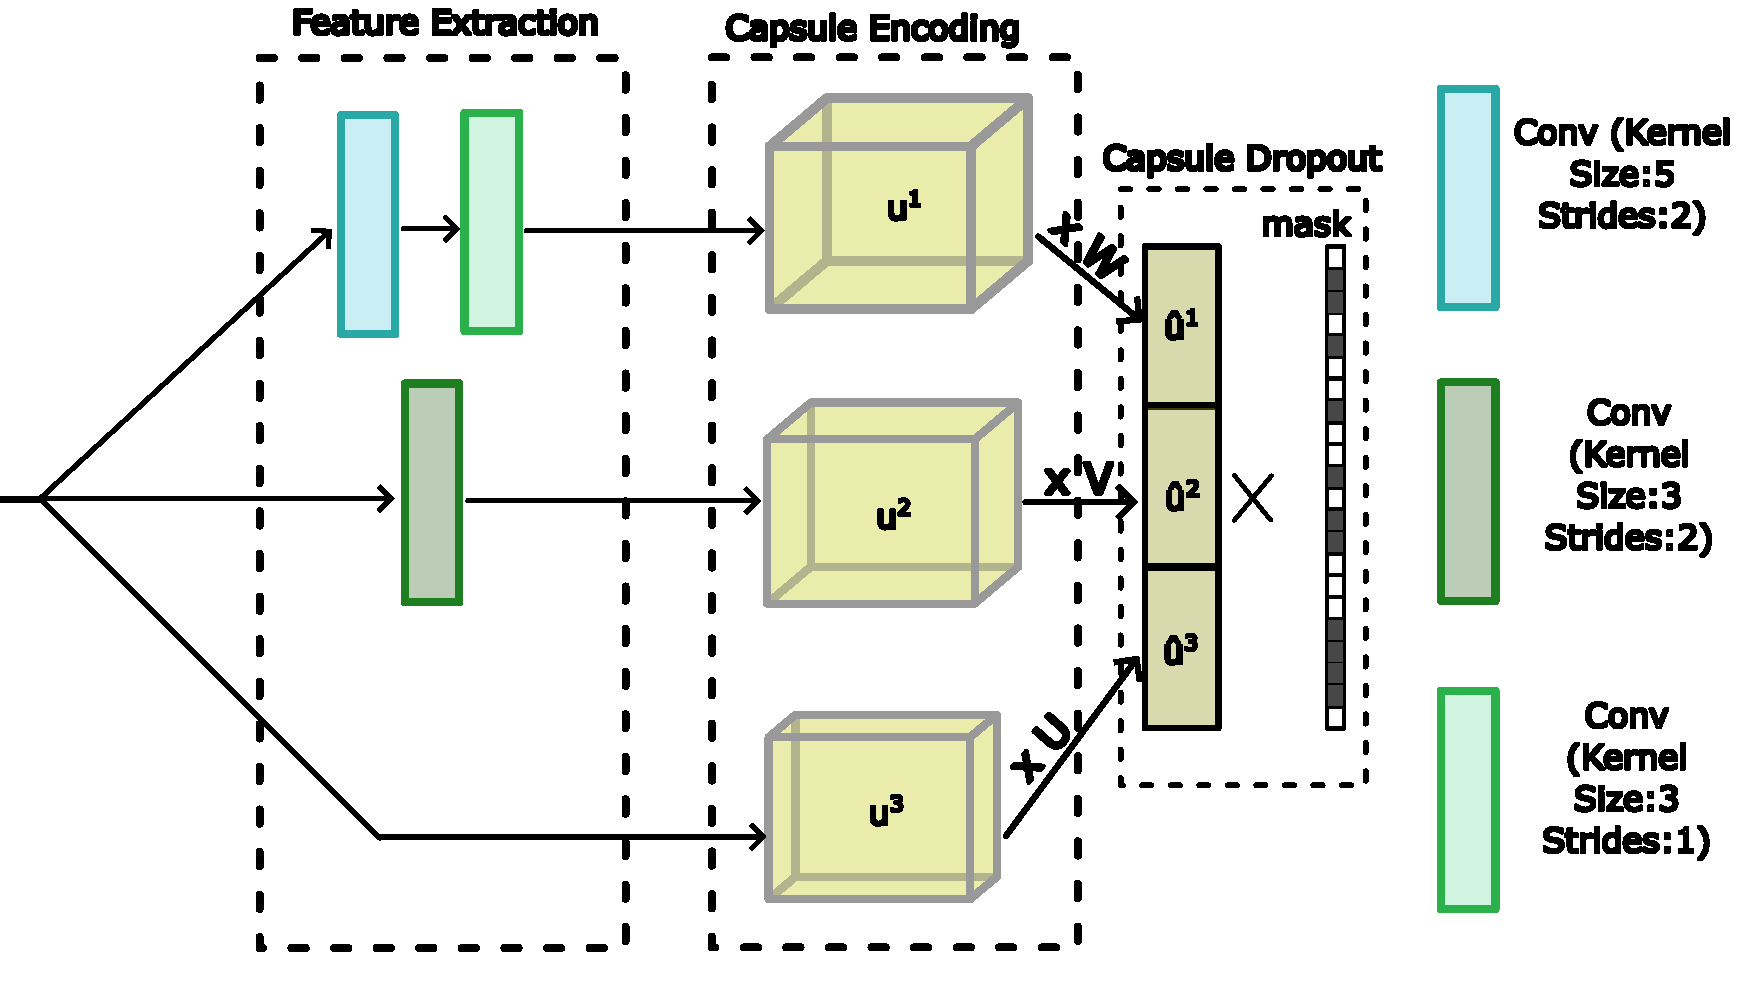
\includegraphics[width=0.8\textwidth]{images/chapter realted work/ms_capsnet.pdf}
    \caption{Αρχιτεκτονική πολυ\textendash κλιμακωτού νευρωνικού δικτύου με κάψουλες \textit{Παράχθηκε από το \href{https://inkscape.org/}{\en{Inkscape}}}.}
    \label{fig:ms_capsnet}
\end{figure}

Η αρχιτεκτονική του πρώτου και δεύτερου επιπέδου του δικτύου φαίνεται στο σχήμα \ref{fig:ms_capsnet}. Έπειτα ακολουθεί το τελευταίο επίπεδο από κάψουλες (παρόμοια με το έργο \cite{sabour2017dynamic}). Χωρίς να εμβαθύνουμε ιδιαίτερα, η εξαγωγή χαρακτηριστικών γίνεται πολυκλιμακωτά, με το πρώτο παρακλάδι να παράγει κωδικοποιήσεις σημασιολογικής πληροφορίας (πληροφορίας ανώτερης τάξης), το δεύτερο να παράγει διανύσματα που κωδικοποιούν πληροφορία μέσης τάξης και το τελευταίο, να έχει ως έξοδο τα ακατέργαστα χαρακτηριστικά. Τα εξαγόμενα χαρακτηριστικά οργανώνονται σε κάψουλες που εμπεριέχουν διανύσματα διαστατικότητας 12, 8 και 4 αντίστοιχα (ανάλογα με το παρακλάδι από το οποίο προκύπτουν). Τέλος, μέσω των πινάκων μετασχηματισμών $W, V, U$, παράγονται ψήφοι ίσου μεγέθους  $\hat{u^1_{j|i}}, \hat{u^2_{j|i}}, \hat{u^3_{j|i}}$ για κάθε ζεύγος $i \rightarrow j$ που συνδέονται σηρειακά (\en{concatenate}) σε ένα διάνυσμα $\hat{u_{j|i}} = concat(\hat{u^1_{j|i}}, \hat{u^2_{j|i}}, \hat{u^3_{j|i}})$.\par

Δυστυχώς, πέρα από τα προαναφερθέντα πειράματα, το δίκτυο δεν εξετάζεται κατά πόσον τηρεί τις θεμελιώδεις υποθέσεις των νευρωνικών δικτύων με κάψουλες. Επιπλέον, οι πίνακες $W, V, U$ δεν έχουν τετραγωνική μορφή με αποτέλεσμα να μην είναι αναστρέψιμοι (και κατά συνέπεια, ο μετασχηματισμός δεν είναι γεωμετρικός).

\subsubsection{\en{DDRM-CapsNet: Capsule Network Based on Deep Dynamic Routing Mechanism for Complex Data}}

Στο έργο των \en{Liu et al.} \footnote{Σε ελεύθερη μετάφραση: \textquote{Νευρωνικό Δίκτυο από Κάψουλες Βασισμένο πάνω σε Βαθύ Δυναμικό Μηχανισμό Δρομολόγησης για Σύνθετα Δεδομένα}.} \cite{liu2019ddrm} δοκιμάζεται μια πιο σύνθετη αρχιτεκτονική με περισσότερες παραμέτρους προκειμένου το δίκτυο να ανταποκρίνεται καλύτερα σε πιο σύνθετα σύνολα δεδομένων. Συγκεκριμένα, πειραματίζονται με διάφορες αρχιτεκτονικές που εισάγουν ένα, δύο, τρία ή τέσσερα συνελικτικά επίπεδα πριν το πρώτο επίπεδο από κάψουλες (\en{PrimaryCaps}). Επιπλέον, εισάγουν ένα ακόμα επίπεδο από κάψουλες τύπου \en{DigitCaps} με αποτέλεσμα ο (υπολογιστικά κοστοβόρος) αλγόριθμος δρομολόγησης να πρέπει να εφαρμοστεί δύο φορές κατά ένα πρόσθιο πέρασμα. Ακόμη, αυξάνουν την εκφραστικότητα της κάθε κάψουλας με την αύξηση της διάστασης του διανύσματος χαρακτηριστικών που ενθυλακώνουν.\par

Μετά από πειράματα, κατέληξαν στη βέλτιστη αρχιτεκτονική η οποία περιλαμβάνει τρία συνελικτικά επίπεδα και τρία επίπεδα από κάψουλες με το τελευταίο επίπεδο να έχει κάψουλες με μεγαλύτερα σε μήκος διανύσματα ($D=24$). Χρησιμοποιώντας αυτή την παραμετροποίηση επιτεύχθηκε μεταξύ άλλων ακρίβεια 77.5\% στο σύνολο δεδομένων \en{CIFAR10} και 29.93\% ακρίβεια στο σύνολο \en{CIFAR100} (επιδώσεις βελτιωμένες κατά 11\% και 8\% αντίστοιχα σε σχέση με το \cite{sabour2017dynamic}). Βέβαια, όλα αυτά γίνονται με αυξημένο υπολογιστικό κόστος και χωρίς να δοκιμάζεται αν συνεχίζουν να τηρούνται οι βασικές υποθέσεις των νευρωνικών δικτύων με κάψουλες.

\subsubsection{\en{DeepCapsnet: Going Deeper with Capsule Networks}}

Στο έργο των \en{Rajasegaran et al.} \footnote{Σε ελεύθερη μετάφραση: \textquote{Πηγαίνοντας Βαθύτερα με τα Νευρωνικά Δίκτυα από Κάψουλες}.} \cite{rajasegaran2019deepcaps} εισάγεται μια νέα αρχιτεκτονική προκειμένου να ανταποκρίνεται καλύτερα σε πιο σύνθετα δεδομένα. Η αρχιτεκτονική αυτή χρησιμοποιεί υπολειμματικές συνδέσεις (\en{residual connections}), ένα δίκτυο αποκωδικοποιητή ως μέθοδο ομαλοποίησης (\en{regularization}) και αποφυγής υπερπροσαρμογής (\en{overfitting}) που δέχεται μόνο το διάνυσμα της προβλεφθείσας κλάσης και ένα δυναμικό αλγόριθμο δρομολόγησης εμπνευσμένο από τρισδιάστατες συνελίξεις (\en{3D convolutions}). \par

Τα πειραματικά αποτελέσματα δείχνουν ότι το μοντέλο, συγκρινόμενο -μεταξύ άλλων- με το έργο \cite{sabour2017dynamic} επιτυγχάνει ελαφρώς καλύτερα αποτελέσματα στα δεδομένων (\en{CIFAR10, SVHN} και \en{FashionMNIST}) με λιγότερες παραμέτρους (λόγω του διαμοιρασμού παραμέτρων που προσφέρει η συνέλιξη). Επίσης, μειώνουν το υπολογιστικό κόστος του δυναμικού αλγορίθμου δρομολόγησης που αναπτύσσουν μειώνοντάς τον αριθμό των επαναλήψεων δρομολόγησης. Τέλος, παρατηρείται μια συνοχή στο τι αναπαριστά το κάθε στοιχείο του διανύσματος χαρακτηριστικών (των καψουλών του τελευταίου επιπέδου), ανεξαρτήτως κλάσης. Για παράδειγμα, το $28^\circ$ στοιχείο του διανύσματος φαίνεται να επηρεάζει την κάθετη επιμήκυνση του ψηφίου, ανεξάρτητα από την κάψουλα εξόδου (και την κλάση του ψηφίου). \par

Αν και ο αλγόριθμος δρομολόγησης και η αρχιτεκτονική του προτεινόμενου δικτύου είναι αρκετά διαφορετική από τη βασική υλοποίηση \cite{sabour2017dynamic}, δεν έγιναν πειράματα που να αποδεικνύουν ότι οι βασικές ιδιότητες των νευρωνικών δικτύων με κάψουλες διατηρούνται. Μάλιστα, στην απλή περίπτωση του συνόλου δεδομένων \en{MNIST}, η επίδοση είναι πιο περιορισμένη.

\subsubsection{\en{FSC\textendash CapsNet: Fractionally\textendash Strided Convolutional Capsule Network for complex data}}

Στο έργο των \en{Liu et al.} \footnote{Σε ελεύθερη μετάφραση: \textquote{Νευρωνικά Δίκτυα με Κάψουλες Κλασματικού Βηματισμού για Σύνθετα Δεδομένα}.} \cite{liu2019fsc} προτείνεται μια νέα αρχιτεκτονική η οποία βελτιώνει τόσο το κύριο μέρος του νευρωνικού δικτύου όσο και τον αποκωδικοποιητή. Πιο συγκεκριμένα, αυξάνεται ο αριθμός των συνελικτικών επιπέδων πριν από το πρώτο επίπεδο από κάψουλες προκειμένου να εξάγονται πιο πλούσια χαρακτηριστικά. Επιπρόσθετα, αναφορικά με τον αποκωδικοποιητή, χρησιμοποιούνται συνελικτικά επίπεδα κλιμακωτού βηματισμού (\en{fractionally\textendash strided convolutional layers}) που αποσκοπούν να βελτιώσουν την ποιότητα των ανακατασκευασμένων εικόνων. \par

Μέσα από πειράματα σε πέντε σύνολα δεδομένων επιλέχθηκε η βέλτιστη παραλλαγή της προτεινόμενης αρχιτεκτονικής η οποία αποτελείται από τρία συνελικτικά επίπεδα (που προηγούνται του πρώτου επιπέδου από κάψουλες) και δύο συνελικτικά επίπεδα κλιμακωτού βηματισμού (\en{fractionally\textendash strided convolutional layers}). Ενδεικτικά για τα πειραματικά αποτελέσματα, στο \en{CIFAR10} επιτεύχθηκε ποσοστό ακρίβειας 77.53\% ενώ στο \en{CIFAR100} το αντίστοιχο ποσοστό ήταν 25.83\%. Ακόμα, παρατηρήθηκε (οπτικά) καλύτερη ανακατασκευή των εικόνων λόγω του βελτιωμένου αποκωδικοποιητή. Δυστυχώς, δεν έγιναν τα απαραίτητα πειράματα για να διασφαλιστεί ότι οι ιδιότητες των νευρωνικών δικτύων με κάψουλες διατηρούνται (\en{invariance on capsule activations, equivariance on capsule poses}).

\subsubsection{\en{Self\textendash Attention Capsule Networks for Object Classification}}

Στο έργο των \en{Hoogi et al.} \footnote{Σε ελεύθερη μετάφραση: \textquote{Νευρωνικά Δίκτυα με Κάψουλες και Μηχανισμό Αυτο\textendash προσοχής για την Ταξινόμηση Αντικειμένων}.} \cite{hoogi2019self} παρουσιάζεται μια πρωτότυπη αρχιτεκτονική νευρωνικών δικτύων με κάψουλες η οποία ενσωματώνει μηχανισμό αυτο\textendash προσοχής. Αναλυτικότερα, μεταξύ του συνελικτικού επιπέδου και του πρώτου επιπέδου από κάψουλες παρευρίσκεται ένα επίπεδο που υλοποιεί τον μηχανισμό αυτο\textendash προσοχής, όπως τον περιγράψαμε στην ενότητα \ref{sec:transformers}. Με αυτόν τον τρόπο, βελτιώνεται η αρχιτεκτονική του νευρωνικού δικτύου χωρίς να αυξάνεται σημαντικά η υπολογιστική πολυπλοκότητα του δικτύου.\par

Η προτεινόμενη αρχιτεκτονική δοκιμάστηκε σε έξι σύνολα δεδομένων, τα τρία εκ των οποίων αποτελούν σύνολα από ιατρικές εικόνες. Αναλυτικότερα για το διαδεδομένο σύνολο δεδομένων \en{CIFAR10}, παρατηρήθηκε 3.55\% βελτίωση σε σχέση με την υλοποίηση στο \cite{sabour2017dynamic} ενώ στο σύνολο δεδομένων \en{MNIST} δεν παρατηρήθηκε κάποια αξιοσημείωτη βελτίωση. Είναι σημαντικό να επισημάνουμε ότι το μοντέλο δε δοκιμάστηκε σε σύνολα δεδομένων όπως το \en{affNIST} και συνεπώς δεν μπορούμε να εγγυηθούμε τη διατήρηση των θεμελιωδών ιδιοτήτων σχετικά με την ικανότητά τους να γενικεύουν σε νέες οπτικές γωνίες.

\subsubsection{\en{DA\textendash CapsNet: Dual Attention Mechanism Capsule Network}}

Στη μελέτη των \en{Huang W.} και \en{Zhou F.} \footnote{Σε ελεύθερη μετάφραση: \textquote{Νευρωνικά Δίκτυα με Κάψουλες και Διπλό Μηχανισμό Προσοχής}.} \cite{huang2020capsnet} δοκιμάζεται μια αρχιτεκτονική νευρωνικών δικτύων με κάψουλες που περιέχει διπλό μηχανισμό προσοχής. Αναλυτικότερα, εφαρμόζεται μηχανισμός προσοχής τόσο μεταξύ των συνελικτικών επιπέδων και του πρώτου επιπέδου από κάψουλες (ονομάζεται \en{Conv\textendash Attention}) όσο και μεταξύ του πρώτου επιπέδου από κάψουλες (\en{PrimaryCaps}) και του τελευταίου επιπέδου από κάψουλες (ο συγκεκριμένος μηχανισμός διαφέρει από το ν προηγούμενο και ονομάζεται \en{Caps\textendash Attention}). Αναφορικά με τον πρώτο, μοιάζει περισσότερο με ένα επίπεδο προσοχής το οποίο γίνεται στους διαφορετικούς χάρτες χαρακτηριστικών (στα κανάλια) αφού η εξαγωγή των βαρών προσοχής περιλαμβάνει τη μέση συνάθροιση (\en{average pooling}) με πυρήνα το πλάτος και ύψος των χαρτών χαρακτηριστικών. Αναφορικά με το δεύτερο μηχανισμό προσοχής, περιλαμβάνει εκπαιδευόμενα βάρη προσοχής που εφαρμόζονται ανά 10 κάψουλες. Μετά από την εφαρμογή του \en{Caps\textendash Attention}, σχηματίζονται άλλες κάψουλες που συμμετέχουν στον μηχανισμό δυναμικής δρομολόγησης, όπως περιγράφεται στο \cite{sabour2017dynamic}.\par

Ο διπλός μηχανισμός προσοχής που ενσωματώνεται στο προτεινόμενο μοντέλο αποσκοπεί στη βελτίωση της αξίας της πληροφορίας που περιγράφεται από τις κάψουλες, στην ελάττωση της περιττής πληροφορίας και στη βελτίωση της ιεραρχίας των καψουλών. Αποδεικνύεται (με μια διαδικασία που προσομοιάζει \en{ablation study}) ότι ο διπλός μηχανισμός προσοχής οδηγεί σε καλύτερα πειραματικά αποτελέσματα σε σχέση με άλλες παραλλαγές νευρωνικών δικτύων με κάψουλες που χρησιμοποιούν μονό μηχανισμό προσοχής. Το δίκτυο δοκιμάζεται σε έξι σύνολα δεδομένων και παρουσιάζει σε όλα βελτιωμένη απόδοση σε σχέση με τη βασική υλοποίηση του \cite{sabour2017dynamic}. Ενδεικτικά, στα σύνολα δεδομένων \en{MNIST, CIFAR10} και \en{smallNORB} παρατηρούνται ποσοστά ακρίβειας ταξινόμησης 99.53, 85.47 και 98.26 αντίστοιχα. Κλείνοντας, αξίζει να σημειώσουμε πως αν και το μοντέλο δοκιμάστηκε στο σύνολο δεδομένων \en{smallNORB}, δεν εξετάστηκε η ικανότητα γενίκευσης σε νέες οπτικές γωνίες, για τις οποίες δεν έχει εκπαιδευτεί.

\subsubsection{\en{Quick\textendash CapsNet (QCN): A Fast Alternative to Capsule Networks}}

Στη μελέτη των \en{Shiri et al.} \footnote{Σε ελεύθερη μετάφραση: \textquote{Μια Ταχεία Εναλλακτική των Νευρωνικών Δικτύων με Κάψουλες}.} \cite{shiri2020quick} αναγνωρίζεται η αδυναμία των νευρωνικών δικτύων με κάψουλες αναφορικά με την ταχύτητα εκπαίδευσης και πρόβλεψης. Για τον σκοπό αυτό γίνονται μια σειρά από πειράματα για τη βελτίωση του υπολογιστικού κόστους με όσο το δυνατόν μικρότερη επίπτωση στις επιδόσεις ταξινόμησης. Αναλυτικότερα, αν εξαιρέσουμε τον (προαιρετικό) αποκωδικοποιητή ανεξαρτήτου\textendash κλάσης (\en{class\textendash independent}) που περιλαμβάνει συνελικτικά επίπεδα κλιμακωτού βηματισμού (\en{fractionally\textendash strided convolutional layers}) και την αντικατάσταση του δευτέρου συνελικτικού επιπέδου με ένα πλήρως διασυνδεδεμένο επίπεδο, δεν προτείνεται κάποια άλλη τροποποίηση της αρχιτεκτονικής ή του αλγορίθμου δρομολόγησης επί της βασική υλοποίησης. Με άλλα λόγια, η ελάττωση του υπολογιστικού κόστους βασίζεται στη μεταβολή των υπερπαραμέτρων της βασικής υλοποίησης όπως περιγράφεται στο \cite{sabour2017dynamic}. 

Μετά από την παρατήρηση ότι ο αριθμός των καψουλών επηρεάζει καθοριστικά την πολυπλοκότητα του δικτύου, έγιναν πειράματα σε σύνολα δεδομένων (\en{MNIST, FashionMNIST, SVHN, CIFAR10, affNIST}) ύστερα από τον περιορισμό του αριθμού των καψουλών του πρώτου επιπέδου (\en{PrimaryCaps}) από 1152 που είναι στη βασική υλοποίηση σε 8 είτε 6 είτε 4. Παρατηρήθηκε ότι αν και υπήρξε ελάττωση της ακρίβειας, οι χρόνοι εκπαίδευσης και πρόβλεψης αυξάνονταν σημαντικά. Ενδεικτικά, για το σύνολο δεδομένων \en{MNIST} και για την παραλλαγή που χρησιμοποιεί μόλις έξι πρωταρχικές κάψουλες (\en{PrimaryCaps}) και βελτιωμένο αποκωδικοποιητή, η ακρίβεια έπεσε από 99.47\% σε 99.19\% ενώ η ταχύτητα εκπαίδευσης και πρόβλεψης αυξήθηκε κατά 5.5 φορές. Τέλος, έγιναν πειράματα για να διασφαλιστεί η ευρωστία του προτεινόμενου μοντέλου στους αφινικούς μετασχηματισμούς - βασική ιδιότητα των νευρωνικών δικτύων με κάψουλες. Στα πειράματα αυτά, παρατηρήθηκε μια πτώση ακρίβειας ταξινόμησης της τάξης του 10\%.

\subsubsection{\en{CapsNet vs CNN: Analysis of the Effects of Varying Feature Arrangement}}

Το έργο των \en{Manogaran et al.} \footnote{Σε ελεύθερη μετάφραση: \textquote{\en{CapsNet vs CNN:} Ανάλυση της Επίδρασης της Διακύμανσης της Χωρικής Διαρρύθμισης των Χαρακτηριστικών}.} \cite{manogaran2020capsnet} εξετάζει την εγκυρότητα της βασικής υπόθεσης ότι τα νευρωνικά δίκτυα με κάψουλες μπορούν να διαχειρίζονται καλύτερα τις σχέσεις μερών\textendash όλου και δεν υποφέρουν από το \textquote{πρόβλημα του \en{Picasso}}. Για την εξέταση της υπόθεσης αυτής, κατασκευάζονται δύο απλά σύνολα δεδομένων. Το πρώτο αποτελείται από παραλληλόγραμμα και ισόπλευρα τρίγωνα. Το δεύτερο, αποτελείται από συνδυασμούς των δύο απλών αντικειμένων (ή μερών) που προαναφέραμε για τη σύνθεση αντικειμένων που είναι βέλη και μη\textendash βέλη (τα μη βέλη προκύπτουν από τυχαίες διατάξεις ενός ορθογώνιου παραλληλογράμμου και ενός τριγώνου). Στη συνέχεια, ένα συνελικτικό δίκτυο και ένα νευρωνικό δίκτυο με κάψουλες (όπως περιγράφεται στο έργο \cite{sabour2017dynamic} αφού τροποποιήθηκε κατάλληλα) εκπαιδεύτηκαν στο πρώτο σύνολο δεδομένων. Έτσι, τα συνελικτικά επίπεδα των δύο δικτύων έμαθαν να αναγνωρίζουν τα επιμέρους αντικείμενα (τρίγωνα και ορθογώνια παραλληλόγραμμα). Έπειτα, παγώνοντας (\en{freeze}) τα συνελικτικά επίπεδα, τα δύο δίκτυα μετεκπαιδεύτηκαν στο δεύτερο σύνολο δεδομένων στο οποίο και τελικά εξετάστηκαν. Από τα πειράματα προέκυψε ότι τα συνελικτικά δίκτυα μπορούσαν καλύτερα να διακρίνουν τα βέλη από τα μη\textendash βέλη σε σχέση με τα νευρωνικά δίκτυα από κάψουλες. Δηλαδή, μπορούσαν να διαχειρίζονται καλύτερα τις σχέσεις μερών (ορθογώνιων παραλληλογράμμων και τριγώνων) και αντικειμένων (βελών). Αυτό είναι μια ένδειξη που κλονίζει μια από τις συνηθισμένες υποθέσεις των νευρωνικών δικτύων από κάψουλες. Παρόλα αυτά, σύμφωνα με τους συγγραφείς, είναι πιθανό το προτέρημα των συνελικτικών νευρωνικών δικτύων να πηγάζει από την απλότητα του συνόλου δεδομένων.


\subsubsection{\en{R\textendash CapsNet: An Improvement of Capsule Network for More Complex Data}}

Το έργο των \en{Luo et al.} \footnote{Σε ελεύθερη μετάφραση: \textquote{Μια Βελτίωση των Νευρωνικών Δικτύων με Κάψουλες για Σύνθετα Δεδομένα}.} \cite{luo2019r} προτείνει μια αποδοτική αρχιτεκτονική νευρωνικού δικτύου με 45\% λιγότερες παραμέτρους από αυτήν που περιγράφεται στο \cite{sabour2017dynamic}. Το επιτυγχάνει αυτό εισάγοντας ένα επιπλέον συνελικτικό επίπεδο και μειώνοντας το μέγεθος των πυρήνων συνέλιξης (\en{convolution kernels}). Αναφορικά με τα πειράματα, δοκιμάζεται στα σύνολα δεδομένων \en{CIFAR10} και \en{FashionMNIST}. Στο τελευταίο, η επίδοση στο σύνολο ελέγχου ανέρχεται στο 93.89\% (έναντι 92.57\% της βασικής υλοποίησης \cite{sabour2017dynamic}). Δυστυχώς, δε γίνεται λόγος για πειράματα που εξετάζουν τη διατήρηση των βασικών υποθέσεων της εν λόγω τεχνολογίας νευρωνικών δικτύων.

\subsubsection{\en{CapsNet Based on Encoder and Decoder for Object Detection}}

Στο έργο των \en{Luo et al.} \footnote{Σε ελεύθερη μετάφραση: \textquote{Νευρωνικό Δίκτυο με Κάψουλες Βασισμένο σε Αρχιτεκτονική Κωδικοποιητή\textendash Αποκωδικοποιητή για την Αναγνώριση Αντικειμένων}.} \cite{luo2020capsnet} εξετάζεται η δυνατότητα μοντελοποίησης της μεταφοράς (\en{translation equivariance}) από νευρωνικά δίκτυα με κάψουλες. Για τον σκοπό αυτό, δίνεται ιδιαίτερη έμφαση στην κατασκευή ενός βελτιωμένου αποκωδικοποιητή (με τη χρήση συνελικτικών επιπέδων κλιμακωτού βηματισμού - \en{fractionally\textendash strided convolutional layers}\footnote{Ονομάζονται στον χώρο των νευρωνικών δικτύων και ως \en{deconvolutions} ή και \en{transposed convolutions}}). Αποδεικνύεται μέσα από πειράματα σε ένα ελαφρός τροποποιημένο σύνολο δεδομένων \en{MNIST} - στο οποίο τα ψηφία τοποθετούνται σε τυχαίες θέσεις πάνω σε ένα μεγάλο \textquote{καμβά} - ότι η πληροφορία που κωδικοποιείται στις παραμέτρους στιγμιοτύπου της κάθε κάψουλας του τελευταίου επιπέδου (\en{DiggitCaps}) εμπεριέχει και τη θέση του ψηφίου στην εικόνα εισόδου. Οι παρατηρήσεις αυτές, ισχύουν και όταν στην εικόνα εισόδου υπάρχουν πολλαπλά ψηφία. Παρόλα αυτά, οι μεταφορές είναι το μόνο είδος μετασχηματισμού στο οποίο το προτεινόμενο δίκτυο δοκιμάζεται (είδος μετασχηματισμού που και τα συνελικτικά νευρωνικά δίκτυα διαχειρίζονται αποδοτικά).

\subsubsection{\en{Efficient\textendash CapsNet: Capsule Network with Self\textendash Attention Routing}}

Η μελέτη των \en{Mazzia et al.} \footnote{Σε ελεύθερη μετάφραση: \textquote{Νευρωνικό Δίκτυο από Κάψουλες με Μηχανισμό Αυτο\textendash Προσοχής}.} \cite{mazzia2021efficient} αντικαθιστά τον αργό, επαναληπτικό αλγόριθμο δρομολόγησης με έναν μηχανισμό αυτο\textendash προσοχής. Μέσα από μια αποδοτική αρχιτεκτονική με πολύ λιγότερες παραμέτρους (160\en{K}) είναι δυνατή η εξαγωγή ισχυρών αναπαραστάσεων (κωδικοποιημένων στα διανύσματα των καψουλών) και η επίτευξη αξιοσημείωτων αποτελεσμάτων σε μια πληθώρα από σύνολα δεδομένων.\par

 Αναλυτικότερα για την αρχιτεκτονική του προτεινόμενου δικτύου, τα πρώτα επίπεδά του συγκροτούνται από τρία συνελικτικά επίπεδα τα οποία ακολουθούνται από ένα επίπεδο διαχωρίσιμης συνέλιξης κατά βάθος (\en{depthwise separable convolution}). Το επίπεδο αυτό μειώνει σημαντικά τον αριθμό των παραμέτρων και συνθέτει τις πρωταρχικές κάψουλες (\en{PrimaryCaps}). Έπειτα ακολουθεί το τελευταίο επίπεδο από κάψουλες \textquote{ψηφίου} (\en{DigitCaps}). Τα διανύσματα των καψουλών αυτών σχηματίζονται μέσω ενός μηχανισμού αυτο\textendash προσοχής (λεπτομέρειες του μηχανισμού αυτού θα περιγραφούν στο επόμενο κεφάλαιο).\par

 Σε ό,τι αφορά το πειραματικό μέρος της μελέτης, χρησιμοποιήθηκαν τα σύνολα δεδομένων \en{MNIST, smallNORB} και \en{MultiMNIST}. Σε αυτά, το ποσοστιαίο σφάλμα ελέγχου ήταν αντίστοιχα 0.26\%, 2.54\% και 5.1\% (χωρίς \en{ensemble}). Τα προαναφερθέντα αποτελέσματα είναι στο ίδιο εύρος με αυτά διαφορετικών υλοποιήσεων των νευρωνικών δικτύων από κάψουλες αλλά χρησιμοποιώντας πολύ λιγότερες παραμέτρους. Αν και τα σύνολα δεδομένων που χρησιμοποιήθηκαν πιστοποιούν ότι ορισμένες ιδιότητες της τεχνολογίας διατηρούνται (π.χ. ευρωστία σε επικαλυπτόμενα αντικείμενα), δεν εξερευνάται η ικανότητα γενίκευσης σε νέες οπτικές γωνίες (για τις οποίες το δίκτυο δεν έχει εκπαιδευτεί). Επιπλέον, όπως θα δούμε στη συνέχεια, ο νέος αλγόριθμος δρομολόγησης που προτείνεται δεν παρέχει ανατροφοδότηση από τις κάψουλες γονείς στις κάψουλες παιδιά (\en{top\textendash down feedback}).

 \subsubsection{\en{Capsule Network Performance on Complex Data}}

Στη μελέτη των \en{Xi et al.} \footnote{Σε ελεύθερη μετάφραση: \textquote{Επίδοση Νευρωνικών Δικτύων με Κάψουλες σε Σύνθετα Δεδομένα}.} \cite{xi2017capsule} παρουσιάζονται τα αποτελέσματα πειραμάτων στα σύνολα δεδομένων \en{CIFAR10} και \en{MNIST} όπως διενεργήθηκαν σε μια σειρά από παραλλαγές της βασική υλοποίησης του νευρωνικού δικτύου με κάψουλες \cite{sabour2017dynamic}. Ενδεικτικά, οι αλλαγές αφορούσαν την προσθήκη επιπλέον συνελικτικών επιπέδων, την προσθήκη επιπλέον επιπέδων από κάψουλες, την αύξηση του αριθμού των καψουλών, την αλλαγή των παραμέτρων της συνάρτησης σφάλματος κ.α. Από τους πειραματισμούς προκύπτει ότι η αύξηση των συνελικτικών επιπέδων οδηγεί σε μια μικρή βελτίωση της επίδοσης ενώ η αύξηση των επιπέδων από κάψουλες έχει το αντίστροφο αποτέλεσμα. Συνολικά, καμία από τις παραλλαγές δεν παρήγαγε αξιοσημείωτα αποτελέσματα.

\subsubsection{\en{Reasearch on Image Classification Based on Capsnet}}

Στο επιστημονικό έργο των \en{Dong Z.} και \en{Lin S.} \footnote{Σε ελεύθερη μετάφραση: \textquote{Έρευνα στην Ταξινόμηση Εικόνων Βασισμένη στα Νευρωνικά Δίκτυα από Κάψουλες}.} \cite{dong2019research} κατασκευάζονται δύο μοντέλα ταξινόμησης εικόνων με το πρώτο να είναι βασισμένο στην τεχνολογία των \textquote{παραδοσιακών} συνελικτικών νευρωνικών δικτύων (που ενσωματώνουν επίπεδα συνάθροισης) και το δεύτερο να είναι ένα δίκτυο από κάψουλες (παρόμοιο με το \cite{sabour2017dynamic}). Μέσα από τα πειράματα, υποστηρίζει τα προτερήματα του δεύτερου μοντέλου ενώ επισημαίνει τα μειονεκτήματά του, όταν το σύνολο δεδομένων γίνεται πιο σύνθετο. 

\subsubsection{\en{An Optimization View on Dynamic Routing Between Capsules}}

Στη μελέτη των \en{Wang D.} και \en{Liu Q.} \footnote{Σε ελεύθερη μετάφραση: \textquote{Μια Βελτίωση του Αλγορίθμου Δυναμικής Δρομολόγησης Μεταξύ Καψουλών}.} \cite{wang2018optimization} επιδιώκεται η χρήση μιας τυπικής, μαθηματικής διατύπωσης για την περιγραφή της στρατηγικής του αλγορίθμου δυναμικής δρομολόγησης μέσω συμφωνίας \cite{sabour2017dynamic}. Πιο αναλυτικά, αποδεικνύει ότι αυτή είναι παρόμοια με την ελαχιστοποίηση του σφάλματος ομαδοποίησης με τη χρήση της μεθόδου κανονικοποίησης \en{KL} επί των συντελεστών σύζευξης (\en{minimizing a standard clustering loss with KL regularization on the coupling probabilities}). Επιπλέον, προτείνει έναν νέο αλγόριθμο δρομολόγησης που, σε ένα περιορισμένο πλαίσιο εφαρμογής, εμφανίζει ορισμένα προτερήματα έναντι του βασικού αλγορίθμου δυναμικής δρομολόγησης.


\subsubsection{\en{Analysis of Capsule Network (Capsnet) Architectures and Applications}}

Το έργο των \en{Pande et al.} \footnote{Σε ελεύθερη μετάφραση: \textquote{Ανάλυση των Αρχιτεκτονικών και Εφαρμογών των Νευρωνικών Δικτύων με Κάψουλες}.} \cite{pande2018analysis} επιχειρεί να συνοψίσει ορισμένες από τις πρόσφατες εξελίξεις των νευρωνικών δικτύων με κάψουλες αλλά και μερικές εφαρμογές τους. Επιπρόσθετα, κάνει αναφορά σε νέες επιτυχίες των συνελικτικών νευρωνικών δικτύων προκειμένου να εμπνεύσει την επιστημονική μελέτη. Από την περιγραφή των βελτιώσεων της βασικής υλοποίησης της εν λόγω τεχνολογίας γίνεται αντιληπτό το μεγάλο εύρος αυτών. Με άλλα λόγια, διαπιστώνεται ότι οι βελτιώσεις εστιάζουν τόσο στην κατασκευή αποδοτικότερου αλγορίθμου δρομολόγησης και μηχανισμού ανακατασκευής εικόνας όσο και στην ποιοτικότερη εξαγωγή χαρακτηριστικών. 


\subsubsection{\en{A Convolutional Neural Network Based on a Capsule Network with Strong Generalization for Bearing Fault Diagnosis}}

Η μελέτη των \en{Zhu et al.} \footnote{Σε ελεύθερη μετάφραση: \textquote{Ένα Νευρωνικό Δίκτυο με Κάψουλες με Ισχυρή Γενίκευση για τη Διάγνωση Σφαλμάτων σε Έδρανα Μηχανών}.} \cite{zhu2019convolutional} περιγράφει την εφαρμογή των νευρωνικών δικτύων με κάψουλες σε ένα σύστημα εποπτείας της υγείας περιστρεφόμενου εξοπλισμού (\en{health condition monitoring system of rotating machinery}). Η καινοτομία της παρούσας εφαρμογής σε ότι αφορά την τεχνολογία των νευρωνικών δικτύων από κάψουλες έγκειται στην ελαφρώς τροποποιημένη αρχιτεκτονική του χρησιμοποιούμενου δικτύου. Αναλυτικότερα, προτείνουν την χρήση ενός μπλόκ έναρξης (\en{inception block}) και επιπλέον χρησιμοποιούν το μήκος του μεγαλύτερου διανύσματος για εργασία παλινδρόμησης (\en{regression task}). Τα πειράματα που διενεργήθηκαν στο πλαίσιο της εφαρμογής αποδεικνύουν ότι οι προτεινόμενες αλλαγές οδηγούν σε καλύτερη γενίκευση.


\subsubsection{\en{Identifying Aggression and Toxicity in Comments using Capsule Network}}

Το έργο των \en{Srivastava et al.} \footnote{Σε ελεύθερη μετάφραση: \textquote{Εντοπίζοντας Επιθετικότητα και Τοξικότητα σε Σχόλια Χρησιμοποιώντας Νευρωνικά Δίκτυα με Κάψουλες}.} \cite{srivastava2018identifying} είναι το μόνο (σύμφωνα με την παρούσα βιβλιογραφική έρευνα) που χρησιμοποιεί νευρωνικά δίκτυα με κάψουλες σε περιβάλλον επεξεργασίας φυσικής γλώσσας. Η αρχιτεκτονική που χρησιμοποιείται έχει την δομή του \cite{sabour2017dynamic} αλλά για την αρχικοποίηση των πρωτεύοντων καψουλών (\en{PrimaryCaps}) αντί για συνελικτικά δίκτυα χρησιμοποιείται \en{LSTM}. Το προτεινόμενο δίκτυο εμφάνισε πολύ ενθαρυντικά αποτελέσματα στο σύνολο δεδομένων \en{Kaggle\textendash toxic comment} (98.46 \en{ROC AUC}).


\section{Νευρωνικά Δίκτυα με Κάψουλες με Μη\textendash Επιβλεπόμενη Μάθηση}

Στην παρούσα ενότητα θα γίνει συνοπτική αναφορά σε ορισμένες παραλλαγές των νευρωνικών δικτύων με κάψουλες οι οποίες ανήκουν στο γενικότερο πλαίσιο της μη\textendash επιβλεπόμενης μάθησης (\en{unsupervised learning}) αλλά και της αυτο\textendash επιβλεπόμενης μάθησης (\en{self\textendash supervised learning}). Οι παρακάτω μελέτες έχουν πραγματοποιηθεί από τον \en{Hinton G.} και την ομάδα του προκειμένου να στρέψουν την τεχνολογία που ανέπτυξαν σε μια νέα κατεύθυνση. Τέλος, να σημειωθεί ότι όλα τα έργα που παρουσιάζονται στην παρούσα ενότητα έπονται χρονικά των τριών βασικών έργων των νευρωνικών δικτύων με κάψουλες σε περιβάλλον επιβλεπόμενης μάθησης.

\subsubsection{\en{Stacked Capsule Atoencoders}}

Η μελέτη των \en{Kosiorek et al.} \footnote{Ο τίτλος του έργου θα μπορούσε να αποδοθεί στα Ελληνικά ως: \textquote{Στοιβαγμένοι Αυτο\textendash κωδικοποιητές με Κάψουλες}.} \cite{kosiorek2019stacked} ορίζει μια καινούρια μέθοδο για την εκμάθηση χαρακτηριστικών (\en{feature learingn}). Αναλυτικότερα, η εκμάθηση εύρωστων αναπαραστάσεων (\en{viewpoint-equivariant representations}) γίνεται με την χρήση ειδικών κωδικοποιητών και δύο αποκωδικοποιητών. Ο πρώτος αποκωδικοποιητής μαθαίνει να αποσυνθέτει τα αντικείμενα εισόδου σε τμήματα (εξάγοντας πληροφορίες για την πιθανότητα ύπαρξης και την πόζα τους) ενώ ο δεύτερος μαθαίνει να συνθέτει τα τμήματα για τον σχηματισμό αντικειμένων.\par

Τα πειράματα που διενεργούνται σε απλά σύνολα δεδομένων είναι αρκετά ενθαρρυντικά. Για παράδειγμα, σε εργασίες μη επιβλεπόμενης ταξινόμησης επιτυγχάνεται ακρίβεια ταξινόμησης 55\% και 98.7\% για τα σύνολα δεδομένων \en{SVHN} και \en{MNIST} αντίστοιχα. Παρόλα αυτά, σε πιο σύνθετα σύνολα δεδομένων (π.χ. \en{CIFAR10}) τα αποτελέσματα δεν είναι το ίδιο ικανοποιητικά. Αυτό οφείλεται στο γεγονός ότι ο πρώτος στη σειρά αποκωδικοποιητής που προαναφέραμε χρησιμοποιεί στάνταρ μοτίβα απλών αντικειμένων (\en{fixed templates}), γεγονός που περιορίζει την δυνατότητα μοντελοποίησης εικόνων πραγματικού κόσμου.

\subsubsection{\en{Umsupervised Part Representation by Flow Capsules}}

Στο έργο των \en{Sabour et al.} \footnote{Ο τίτλος του έργου θα μπορούσε να αποδοθεί στα Ελληνικά ως: \textquote{Μη\textendash επιβλεπόμενη Αναπαράσταση Τμημάτων από Κάψουλες Ροής}.} \cite{pmlr-v139-sabour21a} προτείνεται ένα σύστημα βασισμένο σε αυτο\textendash επιβλεπόμενη μάθηση που αποσκοπεί να βελτιώσει την ποιότητα των περιγραφητων (θέση, σχήμα) των επιμέρους τμημάτων (\en{part descriptors}) που αναπαριστώνται από τις κάψουλες. Το επιτυγχάνει αυτό μέσα από μια σύνθετη αρχιτεκτονική κωδικοποιητή - αποκωδικοποιητή που αξιοποιεί την κίνηση σε διαδοχικά καρέ βίντεο. Πιο συγκεκριμένα, συγκρίνοντας τα διαδοχικά καρέ και παράγοντας ένα οπτικό πεδίο ροής με βάση αυτά επιτυγχάνουν να διακρύνουν τα (κινούμενα) αντικείμενα - μέρη.\par 

Το προτεινόμενο μοντέλο δοκιμάζεται τόσο στην ικανότητά του για μη\textendash επιβλεπόμενη κατάτμηση όσο και στην ικανότητά του για μη\textendash επιβλεπόμενη ταξινόμηση (τροποποιώντας κατάλληλα το δίκτυο σε ένα \en{FlowSCAE}, όπως προκύπτει από τον συνδυασμό του μοντέλου \en{SCAE} με την προτεινόμενη αρχιτεκτονική). Αναφορικά με την πρώτη εργασία, χρησιμοποιήθηκαν τα σύνολα δεδομένων \en{Geo} και \en{Exercise} όπου το σκορ όπως μετρήθηκε χρησιμοποιώντας την μετρική \en{IoU - Intersection over Union} ήταν 0.96 και 0.58 αντίστοιχα. Τέλος, για την μη\textendash επιβλεπόμενη ταξινόμηση, ενδεικτικά έχουμε σκορ 0.79 και 0.99 της Κ \textendash Μέσης ακρίβειας συστάδων για 4 και 100 συστάδες αντίστοιχα (\en{K\textendash Means clustering accuracy where K equals 4 and 100 respectively}).

\subsubsection{\en{Canonical Capsules: Unsupervised Capsles in Canonical Pose}}

Στο έργο των \en{Sun et al.} \footnote{Ο τίτλος του έργου θα μπορούσε να αποδοθεί στα Ελληνικά ως: \textquote{Μη\textendash επιβλεπόμενες Κάψουλες σε Κανονικοποιημένες Πόζες}.} \cite{sun2021canonical} παρουσιάζεται μια μη\textendash επιβλεπόμενη αρχιτεκτονική νευρωνικού δικτύου με κάψουλες για την διαχείριση τρισδιάστατων δεδομένων (\en{3D point\textendash cloud data}). \footnote{Σημειώνουμε ότι εδώ (όπως και στις υπόλοιπες αναφορές της παρούσας ενότητας), οι κάψουλες δεν έχουν την ίδια δομή με αυτές που παρουσιάστηκαν στην ενότητα \ref{sec:capsule_theory}. Συνήθως, περιέχουν πληροφορία για τόσο για την πόζα του αντικειμένου (θέση ή και προσανατολισμό) και το σχήμα του.} Μέσω μιας αρχιτεκτονικής κωδικοποιητή - αποκωδικοποιητή γίνεται εφικτή η αποσύνθεηση τρισδιάστατων εικόνων σε τμήματα διατηρώντας επιθυμητές ιδιότητες της αναγνώρισης αντικειμένων σε νέες οπτικές γωνίες (\en{invariance - equivariance}). Επίσης, γίνεται εφικτή η έμμεση εκμάθηση ενός μη ρητού (\en{implicit}) συστήματος αναφοράς (\en{frame of referance}) για το κάθε τρισδιάστατο αντικείμενο. Κλείνοντας, σε ότι αφορά το πειραματικό μέρος, το προτεινόμενο μοντέλο επιτυγχάνει βέλτιστη (\en{state-of-the-art}) επίδοση σε εργασίες μη\textendash επιβλεπόμενης ανακατασκευής, ανάθεσης (\en{registration}) και ταξινόμησης. 

\section{Λοιπές Δηοσιεύσεις που Ενέμπνευσαν τις Μεθόδους της Παρούσας Δηπλωματικής}

Την τελευταία ενότητα του παρόντος κεφαλαίου την αφιερώνουμε στην παρουσίαση ορισμένων έργων που δεν σχετίζονται άμεσα με το θέμα της διπλωματικής. Τα έργα αυτά, είτε αφορούν το γενικότερο πρόβλημα της διαχείρισης αντικειμένων υπο νέες οπτικές γωνίες είτε ενέμπνευσαν τις μεθόδους που παρουσιάζουμε στα επόμενα κεφάλαια.

\subsubsection{\en{How to Represent Part\textendash Whole Hierarchies in a Neural Network}}

Η παρούσα μελέτη\footnote{Ο τίτλος του έργου θα μπορούσε να αποδοθεί στα Ελληνικά ως: \textquote{Πώς να Αναπαριστούμε ιεραρχίες Μέρους\textendash Όλου σε ένα Νευρωνικό Δίκτυο}.} \cite{hinton2021represent_GLOM} αφορά τις ιδέες του \en{Hinotn G.} σχετικά με ένα (θεωρητικό) μοντέλο υπολογιστικής όρασης υπό το όνομα \en{GLOM}. Πιο συγκεκριμένα, το μοντέλο συνδυάζει μετασχηματιστές (\en{transformers}), νευρωνικά πεδία (\en{neural fields}), αντιθετική μάθηση (\en{contrastive learning}), νευρωνικά δίκτυα με κάψουλες (\en{capsule networks}), αυτοκωδικοποιητές αποθορυβοποίησης (\en{denoising autoencoders}) και αναδρομικά νευρωνικά δίκτυα (\en{RNNs}). Αυτό το φανταστικό (\en{imaginary}) σύστημα αποσυνθέτει την εικόνα εισόδου σε ένα ιεραρχικό δέντρο (\en{parse tree}) από απεικονιζόμενα αντικείμενα και τα τμήματά τους. Επίσης, να σημειώσουμε ότι το ιεραρχικό δέντρο κατασκευάζεται δυναμικά (ανάλογα με την εκάστοτε εικόνα εισόδου) χωρίς να αλλάζει η αρχιτεκτονική του νευρωνικού δικτύου. Αυτό επιτυγχάνεται με την χρήση ενός πολυβηματικού αλγορίθμου συμφωνίας (\en{multi\textendash step consensus algorithm}) που αναλύει τα σημεία της εικόνας παράλληλα και πολυκλιμακωτά (δηλαδή με διαφορετικά επίπεδα αφαιρετικότητας). Συμπερασματικά, το μοντέλο \en{GLOM} αν και δεν αποτελεί κάποιο υλοποιημένο μοντέλο, αφορά μια ιδέα που αλλάζει ριζικά τον τρόπο κατανόησης (και αναπαράστασης) οπτικών πολυμέσων από τα μοντέρνα συστήματα υπολογιστικής όρασης. 


\subsubsection{\en{GIRAFFE: Representing Scenes as Compositional Generative Neural Feature Fields}}

Το έργο των \en{Niemeyer M.} και \en{Geiger A.}\footnote{Ο τίτλος του έργου θα μπορούσε να αποδοθεί στα Ελληνικά ως: \textquote{Αναπαριστώντας Σκηνές ως Συνθετικά Παραγωγικά Νευρωνικά Πεδία Χαρακτηριστικών}.}\cite{niemeyer2021giraffe} παρουσιάζει ένα παραγωγικό μοντέλο (\en{generative model}) που παρέχει ευελιξία στην σύνθεση (φανταστικών) εικόνων. Πιο συγκεκριμένα, με την εσωτερική αναπαράσταση των σκηνών ως συνθετικά, παραγωγικά, νευρωνικά πεδία χαρακτηριστικών (\en{compositional generative neural feature fields}) είναι δυνατή η απόπλεξη των παραγόντων διακύμανσης (\en{disentangle factors of variation}) όπως για παράδειγμα την ελαχιστοποίηση της αλληλοσυσχέτησης μεταξύ των αντικειμένων σε πρώτο πλάνο και του υπόβαθρου της εικόνας. Έτσι, ο δημιουργός μπορεί να παράξει τεχνικά άρτιες, φανταστικές εικόνες έχοντας έλεγχο στο υπόβαθρο, στα επιμέρους αντικείμενα (και στην γεωμετρία τους) αλλά και στην γωνία θέασης.

\subsubsection{\en{Representing Scenes as Neural Radiance Fields for View Synthesis}}

Στο έργο των \en{Mildenhall et al.} \footnote{Ο τίτλος του έργου θα μπορούσε να αποδοθεί στα Ελληνικά ως: \textquote{Αναπαριστώντας Σκηνές ως Νευρωνικά Ακτινωτά Πεδία για τη Σύνθεση σε Νέες Οπτικές Γωνίες}.}\cite{mildenhall2020nerf} παρουσιάζεται ένα σύστημα το οποίο είναι ικανό, δοσμένων ορισμένων δισδιάστατων εικόνων που αποτελούν προβολές μιας τρισδιάστατης σκηνής, να συνθέτει νέες προβολές υπό γωνίες θέασης που δεν ανήκουν στα δεδομένα εισόδου. Το επιτυγχάνει αυτό ενσωματώνοντας την γνώση για μια σκηνή στα βάρη ενός νευρωνικού δικτύου πρόσθιας τροφοδότησης το οποίο εκπαιδεύεται μέσω της οπισθοδιάδοσης σφάλματως σε μια διαδικασία διαφορικής απόδοσης όγκου (\en{differential volume rendering procedure}). Μετά την εκπαίδευση, το δίκτυο τροφοδοτείται με μια πεντάδα στοιχείων που προσδιορίζουν την θέση και την γωνία λήψης και συνθέτει μια ρεαλιστική προβολή η οποία σέβεται τις δομικές λεπτομέρειες των αντικειμένων της σκηνής καθώς επίσης και τον φωτισμό και τις ανακλάσεις.
